При обработке данных (хранение данных в памяти, передача по каналам связи) существует вероятность битовых ошибок. Они могут возникать из-за альфа частиц от примесей в чипе микросхемы или от нейтронов из фонового космического излучения. Частота единичных битовых ошибок на 1 гигабайт данных составляет от 1 раза в час до 1 раза в тысячелетие. По данным исследования Google получилось, что 1 раз в сутки.
\\Есть несколько способов обработки данных, полученных при передаче с ошибкой:
\begin{itemize}
  \item \emph{Использовать полученные данные без проверки на ошибки.} Для такого способа не нужно выполнять лишних действий. Например, при передаче текста или видеоизображения ошибка в одном блоке (слове, кадре) не исказит общего смысла.
  \item \emph{Обнаружить ошибку, выполнить запрос повторной передачи поврежденного блока.} В случае, если пользователь обнаружил ошибку, потребуется передать не блок, а целое сообщение заново, и при передаче файлов большого размера (видеоизображений, фотоизображений и музыкальных файлов высокого качества) это очень проблематично. Если ошибку обнаружила операционная система, то она обнаружила ее еще при передаче данных, и заново передается только поврежденный блок.
  \item \emph{Обнаружить ошибку и отбросить поврежденный блок.} Как и первый способ, он весьма оправдан при передаче текста или видеоизображений.
  \item \emph{Обнаружить и исправить ошибку.} Не тратится время на повторную передачу данных, но полученные данные корректны. Однако, при таком способе необходимо применять особые методы кодирования и наряду с информационными битами передавать служебные, которые позволяют исправить ошибку.
\end{itemize}
Последний способ характеризует помехоустойчивый код.
\textbf{Помехоустойчивые коды} - это коды, позволяющие обнаружить и (или) исправить ошибки в кодовых словах, которые возникают при передачи по каналам связи.\\
\\\emph{Помехоустойчивое кодирование} предполагает введение в передаваемое сообщение, наряду с информационными, так называемых проверочных разрядов, формируемых в устройствах защиты от ошибок (кодерах-на передающем конце, декодерах — на приемном). Избыточность позволяет отличить разрешенную и запрещенную (искаженную за счет ошибок) комбинации при приеме, иначе одна разрешенная комбинация переходила бы в другую.
\begin{center}
  \textbf{Классификация помехоустойчивых кодов}
\end{center}

\begin{itemize}
\item \textbf{Блочные} - фиксированные блоки информации длиной $k$ символов преобразуются в блоки длиной $n$ символов (независимо друг от друга). Например, при передаче файла объемом в 1 гигабайт он делится на равные блоки по 1 килобайту и каждый килобайт снабжается служебной информацией, которая позволяет понять - корректен данный блок или нет. И при обнаружении некорректного блока передается только он.
    \begin{itemize}
      \item \textbf{Неравномерные} - редко используемые символы кодируются большим количеством символов (имеют большую длину) (азбука Морзе);
      \item \textbf{Равномерные} - длина блока (символа) постоянна (таблица ASCII);
      \begin{itemize}
        \item \textbf{Неразделимые} - коды с постоянной плотностью единиц: информационные и проверочные разряды неразделимы (каждый блок данных на входе получает служебные биты, позволяющие обнаружить ошибки, которые далее не отделяются);
        \item \textbf{Разделимые} - можно отделить (выделить) служебные биты от информационных;
        \begin{itemize}
          \item \textbf{Систематические (линейные)} - циклические коды, биты четности/нечетности, код Хэмминга, код Рида-Соломона, код Боуза-Чоудхури-Хоквингема;
          \item \textbf{Несистематические} - коды с контрольным суммированием;
        \end{itemize}
      \end{itemize}
    \end{itemize}
\item \textbf{Непрерывные} - передаваемая информационная последовательность не разделяется на блоки. Кодирование осуществляется целого потока;
    \begin{itemize}
     \item \textbf{Сверточные} - корректирующие ошибки коды; работают с непрерывным потоком данных, кодируя их при помощи регистров сдвига с линейной обратной связью.
     \end{itemize}
\end{itemize}
\begin{center}
\emph{Помехоустойчивый код характеризуется:}
\end{center}
\begin{itemize}
\item$i$ - числом информационных разрядов;
\item$r$ - числом проверочных разрядов;
\item$n$ - общим числом разрядов ($n = i + r$).
\\\\
\end{itemize}
\emph{\textbf{Коэффициент избыточности:} КИ} = $\frac{r}{n}$.

\section{Кодирование с помощью бита четности}
\textbf{Контрольная сумма (check sum)} - некоторое число, рассчитанное путем применения определенного алгоритма к набору данных и используемое для проверки целостности этого набора данных при их передаче или хранении.
\\
\\\textbf{Бит четности} - частный случай контрольной суммы, представляющий из себя 1 контрольный бит, используемый для проверки четности количества единичных битов в двоичном числе.
\\
\\Контроль некой двоичной последовательности (например, машинного слова) с помощью бита чётности также называют \textbf{контролем по паритету}. Контроль по паритету -- наиболее простой и наименее мощный метод контроля данных.
\\
\\\textbf{Метод расчета бита четности} - суммирование по модулю 2 всех бит числа.
\\
\\\textbf{Сумма по модулю 2} - исключающее "ИЛИ"(для двух операндов), логическое или битовое сложение, разность двух/трех множеств.
\\
\\Обозначение: $A\ mod2\ B = A \oplus B$
\\
\\
\begin{minipage}[l]{3.5cm}
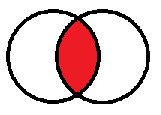
\includegraphics[width=3cm]{6_1_1}
\center{$A \wedge B$}
\end{minipage}
\begin{minipage}[c]{3.5cm}

\includegraphics[width=3cm]{6_1_2}
\center{$A \vee B$}
\end{minipage}
\begin{minipage}[r]{3.5cm}

\includegraphics[width=3cm]{6_1_3}
\center{$A \oplus B$}
\end{minipage}
\\
\\
$A \oplus B = (\neg(A\wedge B))\wedge(A\vee B) = \neg((A\wedge B)\vee(\neg A\wedge \neg B))$
\\
\begin{center}
\textbf{Таблица истинности для $A \oplus B$}
\end{center}
\begin{minipage}[l]{4cm}
\begin{tabular}{|c|c|c|}
\hline
A & B & A $\oplus$ B \\
\hline
0 & 0 & 0 \\
0 & 1 & 1 \\
1 & 0 & 1 \\
1 & 1 & 0 \\
\hline
\end{tabular}
\end{minipage}
\begin{minipage}[l]{6cm}
\begin{tabular}{|c|c|c|c|}
\hline
A & B & C & A $\oplus$ B $\oplus$ C\\
\hline
0 & 0 & 0 & 0 \\
0 & 0 & 1 & 1 \\
0 & 1 & 0 & 1 \\
0 & 1 & 1 & 0 \\
1 & 0 & 0 & 1 \\
1 & 0 & 1 & 0 \\
1 & 1 & 0 & 0 \\
1 & 1 & 1 & 1 \\
\hline
\end{tabular}
\end{minipage}
\\
\\В случае двух переменных результат выполнения операции является истинным тогда и только тогда, когда лишь один из аргументов является истинным.
\\Для функции трех и более переменных результат выполнения операции будет истинным только тогда, когда количество аргументов, равных 1, - нечетное.
\begin{center}
  \textbf{Пример обнаружения ошибок}
\end{center}
Допустим, у нас есть один информационный бит $i = 1$. К нему идет один $r_1$ - бит четности, проверочный разряд №1.
\\$i = r_1$, $i \oplus r_1 = 0$.
\\При получении данных произошел сбой и данные некорректны. Нам известно, что сумма по модулю 2 информационного бита и бита четности равна 0.
\begin{table}[h]
\caption{}
\begin{tabular}{|c|c|c|c|c|}
\hline
i исх & $r_{1}$ исх & i рез & $r_{1}$ рез & i рез $\oplus$ $r_{1}$ рез \\
\hline
1 & 1 & 0 & 0 & 0 \\
1 & 1 & 0 & 1 & 1 \\
1 & 1 & 1 & 0 & 1 \\
1 & 1 & 1 & 1 & 0 \\
\hline
\end{tabular}
\end{table}
\\Соответственно, биты с пометкой "исх"\ - исходные, а "рез"\ - результирующие.
\\В первом случае видно, что несмотря на то, что оба бита пришли с ошибкой, сумма по модулю 2 равна нулю (верна), а значит компьютер не посчитает это как за ошибку.
\\Во втором и третьем случаях сумма по модулю 2 результирующих данных не верна, равна 1. Ошибка.
\\В последнем случае все верно. Биты корректны, сумма по модулю 2 верна. Ошибки нет.
\\
\\Способ обнаружения ошибок с помощью бита четности применяется в RAID-хранилищах (RAID - англ. redundant array of independent disks - избыточный массив независимых дисков) технология виртуализации данных, которая объединяет несколько дисков в логический элемент для избыточности и повышения производительности).

\section{Код Хэмминга}
\begin{wrapfigure}[14]{l}{3 cm}
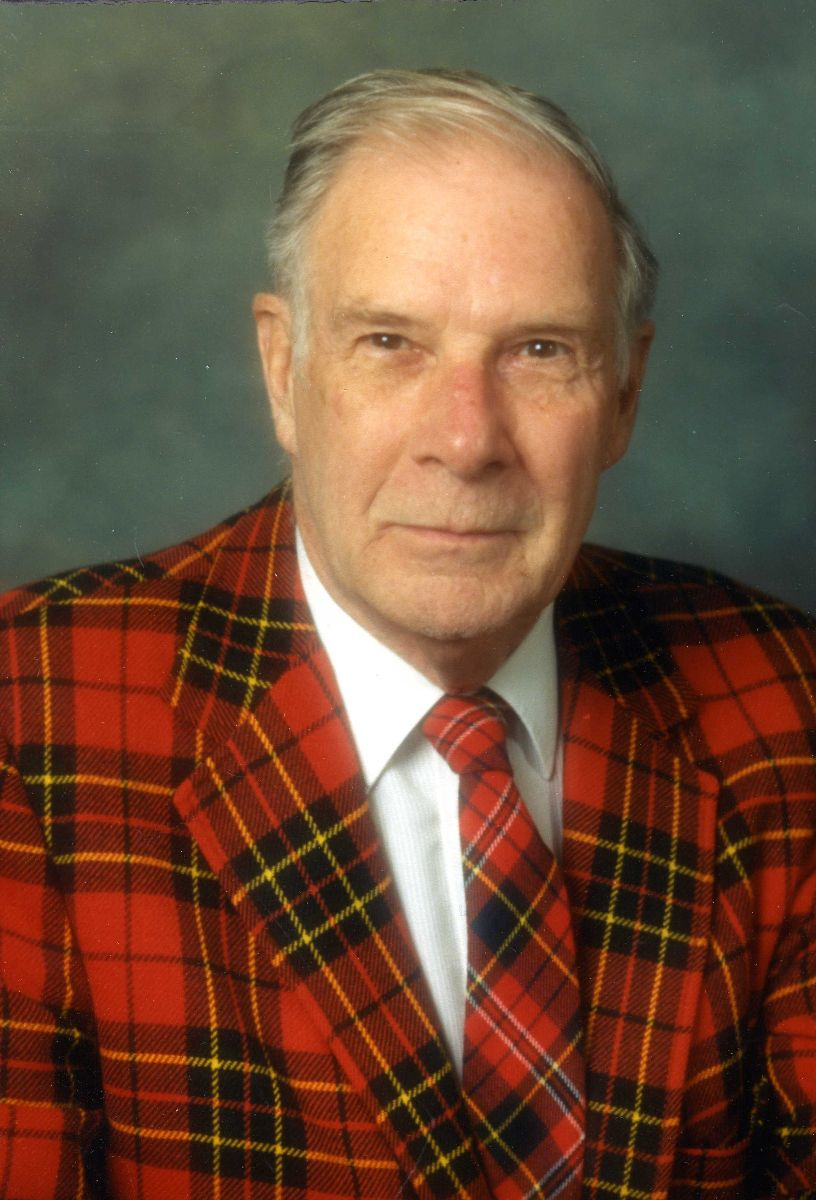
\includegraphics[width=2.5cm]{6_2_1}
\begin{center}
\caption{}
\footnotesize{Р.У. Хэмминг}
\\\footnotesize{$1915 - 1998$}
\end{center}
\end{wrapfigure}
В 1945 году Хэмминг занимался программрованием одного из первых электронных цифровых компьютеров для расчета решения физических уравнений.  В период с 1946 по 1976 года Хэмминг работал в Bell Labs, где сотрудничал с Клодом Шенноном. Хэмминг часто работал в выходные дни, и все больше и больше раздражался, потому что часто был должен перезагружать свою программу из-за ненадежности перфокарт. На протяжении нескольких лет он проводил много времени над построением эффективных алгоритмов исправления ошибок. В 1950 году он опубликовал способ, который на сегодняшний день известен как \emph{код Хэмминга}. \\\\Коды Хэмминга — наиболее известные и, вероятно, первые из \emph{самоконтролирующихся} и \emph{самокорректирующихся} кодов.\\
Рассмотрим подробнее два этих вида кодов:
\begin{itemize}
\item \emph{Самоконтролирующиеся коды} -- коды, позволяющие автоматически обнаруживать ошибки при передаче данных. Для их построения достаточно приписать к каждому слову один добавочный (контрольный) двоичный разряд и выбрать цифру этого разряда так, чтобы общее количество единиц в изображении любого числа было, например, четным. Одиночная ошибка в каком-либо разряде передаваемого слова (в том числе, может быть, и в контрольном разряде) изменит четность общего количества единиц. Счетчики по модулю 2, подсчитывающие количество единиц, которые содержатся среди двоичных цифр числа, могут давать сигнал о наличии ошибок.\\
\\При этом невозможно узнать, в каком именно разряде произошла ошибка, и, следовательно, нет возможности исправить её. Остаются незамеченными также ошибки, возникающие одновременно в двух, в четырёх или вообще в четном количестве разрядов. Впрочем, двойные, а тем более четырёхкратные ошибки полагаются маловероятными;
\item \emph{Самокорректирующиеся коды} -- коды, в которых возможно автоматическое исправление ошибок. Для построения самокорректирующегося кода, рассчитанного на исправление одиночных ошибок, одного контрольного разряда недостаточно. Как видно из дальнейшего, количество контрольных разрядов k должно быть выбрано так, чтобы удовлетворялось неравенство $2^k \ge k+m+1$ или $k \ge log_2{k+m+1}$, где m -  количество основных двоичных разрядов кодового слова. Минимальные значения k при заданных значениях m, найденные в соответствии с этим неравенством, приведены в таблице.

\begin{table}[h]
\caption{}
\begin{center}
\begin{tabular}{|c|c|}
\hline
 Диапазон m & $k_{min}$  \\
\hline
1 & 2 \\
\hline
2-4 & 3\\
\hline
5-11 & 4\\
\hline
12-26 & 5\\
\hline
27-57 & 6 \\
\hline
\end{tabular}
\end{center}
\end{table}
\end{itemize}
В настоящее время наибольший интерес представляют двоичные блочные корректирующие коды. При использовании таких кодов информация передаётся в виде блоков одинаковой длины и каждый блок кодируется и декодируется независимо друг от друга. Почти во всех блочных кодах символы можно разделить на информационные и проверочные. Таким образом, все комбинации кодов разделяются на разрешенные (для которых соотношение информационных и проверочных символов возможно) и запрещенные.\\
\\\textbf{Код Хэмминга} - блочный равномерный разделимый самокорректирующийся код. Исправляет одиночные битовые ошибки, возникшие при передаче или хранении данных.
\\
\\На каждые $i$ информационных бит используется $r$ проверочных.
\\
\\Значение каждого контрольного бита зависит от значений информационных бит: контрольный бит с номером $N$ контролирует все последующие $N$ бит через каждые $N$ бит, начиная с позиции $N$.
\\\textbf{Синдром последовательности S} - набор контрольных сумм информационных и проверочных разрядов.
\\
\\Рассмотрим таблицу:
\begin{table}[h]
\caption{}
\begin{tabular}{|c|c|c|c|c|c|c|c|c|c|c|c|c|c|c|c|}
\hline
& 1 & 2 & 3 & 4 & 5 & 6 & 7 & 8 & 9 & 10 & 11 & 12 & 13 & 14 & \\
\hline
$2^k$ & $r_{1}$ & $r_{2}$ & $i_{1}$ & $r_{3}$ & $i_{2}$ & $i_{3}$ & $i_{4}$ & $r_{4}$ & $i_{5}$ & $i_{6}$ & $i_{7}$ & $i_{8}$ & $i_{9}$ & $i_{10}$ & S\\
\hline
1 & \cellcolor{Gray1}{X} & & \cellcolor{Gray1}{X} & & \cellcolor{Gray1}{X} & & \cellcolor{Gray1}{X} & & \cellcolor{Gray1}{X} & & \cellcolor{Gray1}{X} & & \cellcolor{Gray1}{X} & & $s_{1}$\\
\hline
2 & & \cellcolor{Gray2}{X} & \cellcolor{Gray2}{X} & & & \cellcolor{Gray2}{X} & \cellcolor{Gray2}{X} & & & \cellcolor{Gray2}{X} & \cellcolor{Gray2}{X} & & & \cellcolor{Gray2}{X} & $s_{2}$ \\
\hline
4 & & & & \cellcolor{Gray3}{X} & \cellcolor{Gray3}{X} & \cellcolor{Gray3}{X} & \cellcolor{Gray3}{X} & & & & & \cellcolor{Gray3}{X} & \cellcolor{Gray3}{X} & \cellcolor{Gray3}{X} & $s_{3}$ \\
\hline
8 & & & & & & & & \cellcolor{Gray4}{X} & \cellcolor{Gray4}{X} & \cellcolor{Gray4}{X} & \cellcolor{Gray4}{X} & \cellcolor{Gray4}{X} & \cellcolor{Gray4}{X} & \cellcolor{Gray4}{X} & $s_{4}$ \\
\hline
\end{tabular}
\end{table}
\\Данная таблица представлена для кода из 14 бит, но ее можно расширить для нужного размера самостоятельно.
\\Сверху (в первой строчке) указан номер бита, а справа - синдром.
\\Знаком $X$ обозначены те биты, которые контролирует проверочный бит, с номером, который указан в левом столбце (степень двойки). Чтобы узнать какими битами контролируется бит с номером $N$ надо просто разложить $N$ по степеням двойки.
\\Например, видно, что проверочный бит $r_1$ контролирует информационные биты $i_1$, $i_2$, $i_4$, $i_5$, $i_7$, $i_9$. А 11 бит ($i_7$) контролируется битами 1 ($r_1$), 2 ($r_2$) и 8 ($r_4$).
\\Чтобы узнать значение проверочного бита, необходимо сложить по модулю 2 все информационные биты, которые он контролирует.
\\В данном случае:
\\$r_1 = i_1\oplus i_2\oplus i_4\oplus i_5\oplus i_7\oplus i_9$;
\\$r_2 = i_1\oplus i_3\oplus i_4\oplus i_6\oplus i_7\oplus i_10$;
\\и так далее.
\\Чтобы узнать значение синдрома, необходимо сложить по модулю 2 все биты, которые содержит синдром.
\\В данном случае:
\\$s_1 = r_1\oplus i_1\oplus i_2\oplus i_4\oplus i_5\oplus i_7\oplus i_9$;
\\$s_2 = r_2\oplus i_1\oplus i_3\oplus i_4\oplus i_6\oplus i_7\oplus i_{10}$;
\\и так далее.
\\Синдром последовательности S определяется составляющими синдромами $s_1$, $s_2$ и так далее. То есть для кода, где $r = 3$, синдром будет иметь следующий формат: $S(s_1;s_2;s_3)$.
\\
\\Определение минимального количества контрольных разрядов: $$2^k \ge r + i + 1.$$
\\Классические коды Хэмминга с маркировкой (n, i): (7, 4); (15, 11); (31, 26).
\\
\\Разбрем код Хэмминга для $r = 3$.
\begin{center}
\textbf{Код Хэмминга для $r = 3$}
\end{center}
В данном случае, у нас 7 бит, из них 4 информационных и 3 проверочных. То есть, код имеет маркировку (7, 4).
\\Составим таблицу кода (7, 4):
\begin{table}[h]
\caption{}
\begin{tabular}{|c|c|c|c|c|c|c|c|c|}
\hline
& 1 & 2 & 3 & 4 & 5 & 6 & 7 & \\
\hline
$2^k$ & $r_{1}$ & $r_{2}$ & $i_{1}$ & $r_{3}$ & $i_{2}$ & $i_{3}$ & $i_{4}$ & S\\
\hline
1 & \cellcolor{Gray1}{X} & & \cellcolor{Gray1}{X} & & \cellcolor{Gray1}{X} & & \cellcolor{Gray1}{X} & $s_{1}$\\
\hline
2 & & \cellcolor{Gray2}{X} & \cellcolor{Gray2}{X} & & & \cellcolor{Gray2}{X} & \cellcolor{Gray2}{X} & $s_{2}$ \\
\hline
4 & & & & \cellcolor{Gray3}{X} & \cellcolor{Gray3}{X} & \cellcolor{Gray3}{X} & \cellcolor{Gray3}{X} & $s_{3}$ \\
\hline
\end{tabular}
\end{table}
\\Рассмотрим конкретно контроль информационных бит проверочными на кругах Эйлера:
\\\\
\begin{minipage}[l]{3.5cm}
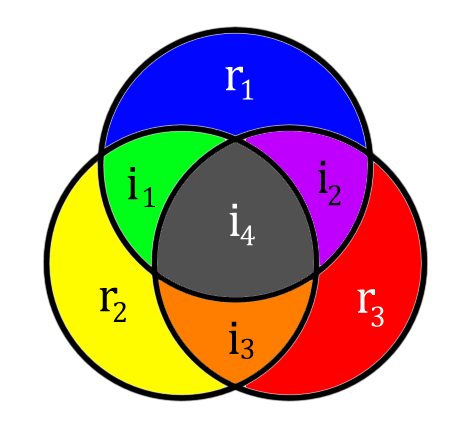
\includegraphics[width=3.5cm]{6_2_2}
\end{minipage}
\begin{minipage}[r]{9cm}
Видно, что $r_1$ контролирует $i_1$, $i_2$ и $i_4$; $r_2$ контролирует $i_1$, $i_3$ и $i_4$; а $r_3$ контролирует $i_2$, $i_3$ и $i_4$.
\\$r_1 = i_1 \oplus i_2 \oplus i_4;$
\\$r_2 = i_1 \oplus i_3 \oplus i_4;$
\\$r_3 = i_2 \oplus i_3 \oplus i_4;$
\end{minipage}
\\
\\$s_1 = r_1 \oplus i_1 \oplus i_2 \oplus i_4;$
\\$s_2 = r_2 \oplus i_1 \oplus i_3 \oplus i_4;$
\\$s_3 = r_3 \oplus i_2 \oplus i_3 \oplus i_4;$
\\
\\Рассмотрим таблицу значений синдрома ($s_1;s_2;s_3$) и позицию ошибочного бита в сообщении.
\begin{table}[h]
\caption{}
\begin{tabular}{|c|c|c|}
\hline
Синдром ($s_1;s_2;s_3$) & Конфигурация ошибок & Ошибочный символ\\
\hline
000 & НЕТ & НЕТ \\
001 & 0001000 & $r_3$ \\
010 & 0100000 & $r_2$ \\
011 & 0000010 & $i_3$ \\
100 & 1000000 & $r_1$ \\
101 & 0000100 & $i_2$ \\
110 & 0010000 & $i_1$ \\
111 & 0000001 & $i_4$ \\
\hline
\end{tabular}
\end{table}\\
Возьмем, к примеру, 2 строку (см. таблицу на следующей странице): синдром $S(0,0,1)$, это значит, что $s_1 = 0$, $s_2 = 0$, $s_3 = 1$. По построенной таблице кода (7,4) определяется, в каком бите ошибка: какой бит содержится только в 3 синдроме. Проще говоря, в каком столбце $X$ стоит только в 3 строчке (напротив $s_3$). По таблице видим, что такой бит - 4 (поэтому во втором столбце 0001000 - нули означают правильный бит, а единица - ошибочный. В данном случае ошибочный бит 4, поэтому он равен единице). Смотрим, какой именно бит занимает четвертое место - $r_3$.
\\Чтобы получить правильную последовательность, необходимо инвертировать ошибочный бит.
\\
\\\emph{\textbf{Пример 1:}}
\\\emph{Задание:} получена последовательность 1100100. Вычислить ошибочный бит, записать правильную последовательность.
\\\emph{Решение:} составим таблицу кода (7,4) с конкретной последовательностью.
\begin{table}[h]
\begin{tabular}{|c|c|c|c|c|c|c|c|c|}
\hline
& 1 & 2 & 3 & 4 & 5 & 6 & 7 & \\
\rowcolor{Gray1}
\hline
& 1 & 1 & 0 & 0 & 1 & 0 & 0 & \\
\hline
$2^k$ & $r_{1}$ & $r_{2}$ & $i_{1}$ & $r_{3}$ & $i_{2}$ & $i_{3}$ & $i_{4}$ & S\\
\hline
1 & \cellcolor{Gray1}{X} & & \cellcolor{Gray1}{X} & & \cellcolor{Gray1}{X} & & \cellcolor{Gray1}{X} & $s_{1}$\\
\hline
2 & & \cellcolor{Gray2}{X} & \cellcolor{Gray2}{X} & & & \cellcolor{Gray2}{X} & \cellcolor{Gray2}{X} & $s_{2}$ \\
\hline
4 & & & & \cellcolor{Gray3}{X} & \cellcolor{Gray3}{X} & \cellcolor{Gray3}{X} & \cellcolor{Gray3}{X} & $s_{3}$ \\
\hline
\end{tabular}
\end{table}
Рассчитаем значение контрольных бит результата:
\\$r_{1\mbox{ рез}} = i_1 \oplus i_2 \oplus i_4 = 0 \oplus 1 \oplus 0 = 1;$
\\$r_{2\mbox{ рез}} = i_1 \oplus i_3 \oplus i_4 = 0 \oplus 0 \oplus 0 = 0;$
\\$r_{3\mbox{ рез}} = i_2 \oplus i_3 \oplus i_4 = 1 \oplus 0 \oplus 0 = 1;$
\\Рассчитаем синдромы:
\\$s_1 = r_1 \oplus i_1 \oplus i_2 \oplus i_4 = r_{1\mbox{ рез}} \oplus r_{1\mbox{ исх}} = 1 \oplus 1 = 0;$
\\$s_2 = r_2 \oplus i_1 \oplus i_3 \oplus i_4 = r_{2\mbox{ рез}} \oplus r_{2\mbox{ исх}} = 0 \oplus 1 = 1;$
\\$s_3 = r_3 \oplus i_2 \oplus i_3 \oplus i_4 = r_{3\mbox{ рез}} \oplus r_{3\mbox{ исх}} = 1 \oplus 0 = 1.$
\\Полученный синдром: $S(0,1,1)$.
\\Смотрим по таблице, какой бит содержится в $s_2$ и $s_3$ одновременно. 6, то есть $i_3$.
\\Инвертируем ошибочный бит и получаем правильную последовательность.
\\Ответ: 6 бит ($i_3$), правильная последовательность: 1100110.
\begin{figure}[h]
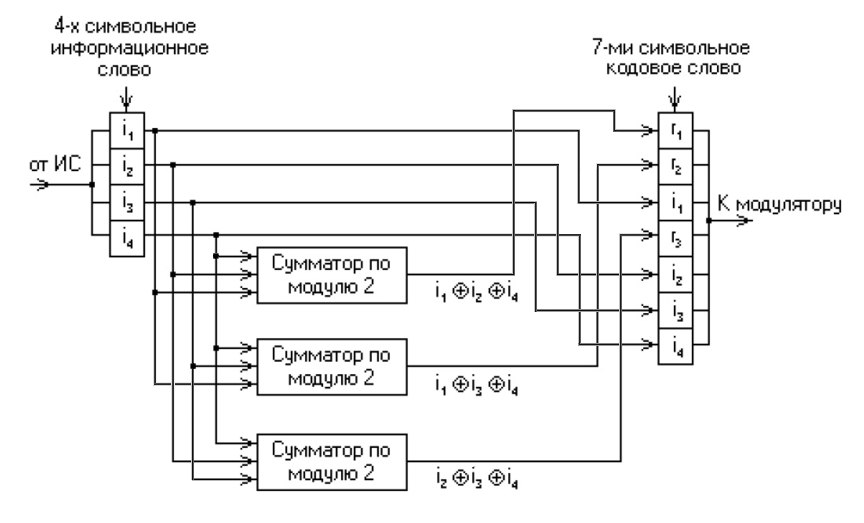
\includegraphics[width=\textwidth]{6_2_3}
\caption{Схема создания кода Хэмминга (7,4)}
\end{figure}
\begin{figure}
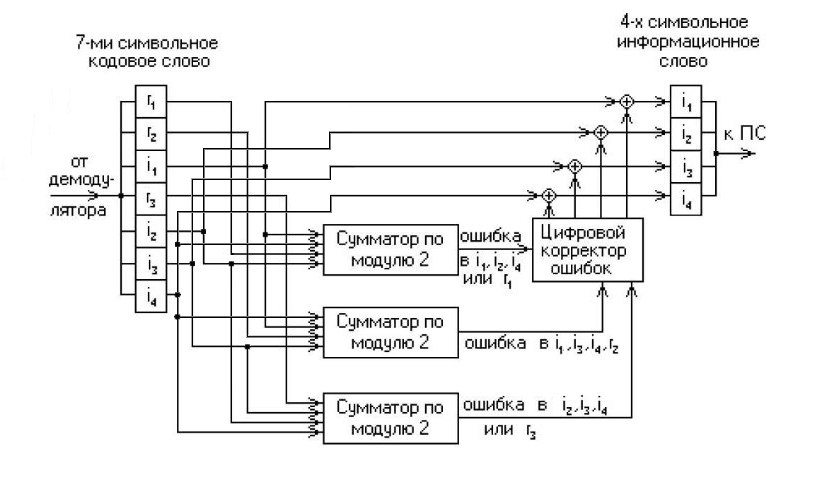
\includegraphics[width=\textwidth]{6_2_4}
\caption{Схема декодирования кода Хэмминга (7,4)}
\end{figure}
\newpage
Разбрем код Хэмминга для $r = 4$ аналогично тому, как мы сделали это выше.
\begin{center}
\textbf{Код Хэмминга для $r = 4$}
\end{center}
В данном случае, у нас 15 бит, из них 11 информационных и 4 проверочных. То есть, код имеет маркировку (15, 11).
\\Составим таблицу кода (15, 11):
\begin{table}[h]
\caption{}
\begin{tabular}{|c|c|c|c|c|c|c|c|c|c|c|c|c|c|c|c|c|}
\hline
& 1 & 2 & 3 & 4 & 5 & 6 & 7 & 8 & 9 & 10 & 11 & 12 & 13 & 14 & 15 & \\
\hline
$2^k$ & $r_{1}$ & $r_{2}$ & $i_{1}$ & $r_{3}$ & $i_{2}$ & $i_{3}$ & $i_{4}$ & $r_{4}$ & $i_{5}$ & $i_{6}$ & $i_{7}$ & $i_{8}$ & $i_{9}$ & $i_{10}$& $i_{11}$ &S\\
\hline
1 & \cellcolor{Gray1}{X} & & \cellcolor{Gray1}{X} & & \cellcolor{Gray1}{X} & & \cellcolor{Gray1}{X} & & \cellcolor{Gray1}{X} & & \cellcolor{Gray1}{X} & & \cellcolor{Gray1}{X} & & \cellcolor{Gray1}{X} & $s_{1}$\\
\hline
2 & & \cellcolor{Gray2}{X} & \cellcolor{Gray2}{X} & & & \cellcolor{Gray2}{X} & \cellcolor{Gray2}{X} & & & \cellcolor{Gray2}{X} & \cellcolor{Gray2}{X} & & & \cellcolor{Gray2}{X} & \cellcolor{Gray2}{X} & $s_{2}$ \\
\hline
4 & & & & \cellcolor{Gray3}{X} & \cellcolor{Gray3}{X} & \cellcolor{Gray3}{X} & \cellcolor{Gray3}{X} & & & & & \cellcolor{Gray3}{X} & \cellcolor{Gray3}{X} & \cellcolor{Gray3}{X} & \cellcolor{Gray3}{X} & $s_{3}$ \\
\hline
8 & & & & & & & & \cellcolor{Gray4}{X} & \cellcolor{Gray4}{X} & \cellcolor{Gray4}{X} & \cellcolor{Gray4}{X} & \cellcolor{Gray4}{X} & \cellcolor{Gray4}{X} & \cellcolor{Gray4}{X} & \cellcolor{Gray4}{X} & $s_{4}$\\
\hline
\end{tabular}
\end{table}
Получим: 
\\$r_1 = i_1 \oplus i_2 \oplus i_4  \oplus i_5  \oplus i_7  \oplus i_9  \oplus i_{11};$ 
\\$r_2 = i_1 \oplus i_3 \oplus i_4  \oplus i_6  \oplus i_7  \oplus i_{10}  \oplus i_{11};$
\\$r_3 = i_2 \oplus i_3 \oplus i_4  \oplus i_8  \oplus i_9  \oplus i_{10}  \oplus i_{11};$
\\$r_4 = i_5 \oplus i_6 \oplus i_7  \oplus i_8  \oplus i_9  \oplus i_{10}  \oplus i_{11};$
\\
\\$s_1 = r_1 \oplus i_1 \oplus i_2 \oplus i_4  \oplus i_5  \oplus i_7  \oplus i_9  \oplus i_{11};$
\\$s_2 = r_2 \oplus i_1 \oplus i_3 \oplus i_4 \oplus i_6  \oplus i_7  \oplus i_{10}  \oplus i_{11};$
\\$s_3 = r_3 \oplus i_2 \oplus i_3 \oplus i_4 \oplus i_8  \oplus i_9  \oplus i_{10}  \oplus i_{11};$
\\$s_4 = r_4 \oplus i_5 \oplus i_6 \oplus i_7  \oplus i_8  \oplus i_9  \oplus i_{10}  \oplus i_{11};$
\\
\\Рассмотрим таблицу значений синдрома ($s_1;s_2;s_3;s_4$) и позицию ошибочного бита в сообщении. \\\\
Рассуждения будут аналогичны. Возьмем, например, 4ую строку (см. таблицу на следующей странице). Синдром S(0,0,1,1) означает, что $s_1 = 0$, $s_2 = 0$, $s_3 = 1$, $s_4 = 1$. По таблице кода (15,11) находится, в каком бите ошибка - какой бит содержится только в 4 синдроме. В данном случае, такой бит - 12. Напомним, что нули обозначают правильный бит, а единица - ошибочный. Двенадцатое место занимает бит $i_8$.

\begin{table}[h]
\caption{Расшифровка сообщений схем 5.2 и 5.3}

\begin{tabular}{|c|c|c|c|}
\hline
Синдром ($s_1;s_2;s_3;s_4$) & Конфигурация ошибок & Ошибочный символ\\
\hline
0000 & НЕТ & НЕТ \\
0001 & $000\ 0000\ 1000\ 0000$ & $r_4$ \\
0010 & $000\ 1000\ 0000\ 0000$ & $r_3$ \\
0011 & $000\ 0000\ 0000\ 1000$ & $i_8$ \\
0100 & $010\ 0000\ 0000\ 0000$ & $r_2$ \\
0101 & $000\ 0000\ 0010\ 0000$ & $i_6$ \\
0110 & $000\ 0010\ 0000\ 0000$ & $i_3$ \\
0111 & $000\ 0000\ 0000\ 0010$ & $i_{10}$\\
1000 & $100\ 0000\ 0000\ 0000$ & $r_1$\\
1001 & $000\ 0000\ 0100\ 0000$ & $i_5$\\
1010 & $000\ 0100\ 0000\ 0000$ & $i_2$\\
1011 & $000\ 0000\ 0000\ 0100$ & $i_9$\\
1100 & $001\ 0000\ 0000\ 0000$ & $i_1$\\
1101 & $000\ 0000\ 0001\ 0000$ & $i_7$\\
1110 & $000\ 0001\ 0000\ 0000$ & $i_4$\\
1111 & $000\ 0000\ 0000\ 0001$ & $i_{11}$\\
\hline
\end{tabular}
\end{table}